\documentclass[letterpaper]{article}
\usepackage{aaai}
\usepackage{times}
\usepackage{helvet}
\usepackage{courier}
\usepackage{amsmath,amsfonts,amssymb,amsthm}
\usepackage{array}
\usepackage{amsmath,amssymb}
\usepackage{epsfig,subfigure}
\usepackage[vlined,algoruled,titlenumbered,noend]{algorithm2e}
\frenchspacing

\newcommand{\MarsRover}{\textsc{Mars Rover}}
\newcommand{\MarsRoverL}{\textsc{Mars Rover Linear}}
\newcommand{\MarsRoverNL}{\textsc{Mars Rover Nonlinear}}
\newcommand{\InventoryControl}{\textsc{Inventory Control}}
\newcommand{\WaterReservoir}{\textsc{Water Reservoir}}
\newcommand{\MultiWaterReservoir}{\textsc{Multi-Reservoir}}
\newtheorem*{example*}{Example}

\newcommand{\true}{\mathit{true}}
\newcommand{\false}{\mathit{false}}
\def\argmax{\operatornamewithlimits{arg\,max}}
\def\argmin{\operatornamewithlimits{arg\,min}}

\setcounter{secnumdepth}{0}  

 \begin{document}
% The file aaai.sty is the style file for AAAI Press 
% proceedings, working notes, and technical reports.
%
\title{Exact Solutions to Continuous State and Action MDPs}
\author{Anonymous}
%\author{Zahra Zamani\\
%NICTA \& the ANU\\
%Canberra, Australia\\
%{\tt zahra.zamani@anu.edu.au}
%\And
%Scott Sanner\\
%NICTA \& the ANU\\
%Canberra, Australia\\
%{\tt ssanner@nicta.com.au}
%\And
%Cheng Feng\\
%Department of Aeronautics and\\
%Astronautics, MIT, USA\\
%{\tt cfang@mit.edu}
%}
\maketitle
\begin{abstract}
\begin{quote}
Many real-world decision-theoretic planning problems are naturally
modeled using both continuous state and action (CSA) spaces.  Previous
work on such problems has only provided exact solutions in limited
settings, leaving one to resort to discretization or sampling as
approximate solution approaches.  In this work, we propose a symbolic
dynamic programming solution to obtain the \emph{optimal closed-form}
value function and policy for CSA-MDPs with discrete noise, piecewise
linear dynamics, and piecewise quadratic rewards.  Crucially we show
how the continuous action maximization step in the dynamic programming
backup can be evaluated optimally and symbolically for this case;
further we extend this maximization operation to work with an
efficient and compact data structure, the extended algebraic decision
diagram (XADD).  We demonstrate empirical results for CSA-MDPs on a
range of domains from planning and operations research to demonstrate
the first \emph{exact solution} to these problems --- even in the case
of multivariate actions and nonlinear reward.
\end{quote}
\end{abstract}

\section{Introduction}

\label{sec:intro}

Many real-world stochastic planning problems involving resources,
time, or spatial configurations naturally use continuous variables in
both their state and action representation.  For example, in a variant
of the
%\InventoryControl problem, a business must must decide how many
%of each item to reorder subject to uncertain demand, inventory holding
%constraints, and quantity-dependent reordering costs.
\MarsRover\ problem~\cite{bresina02}, a rover must navigate within a
continuous environment and carry out assigned scientific discovery
tasks.  In oversubscribed cases where the \MarsRover\ may not be able
to visit all of its assigned landmarks (e.g., to take pictures) within a
given time horizon, it may still be rewarded to some degree for
partial objective fulfillment (e.g, taking pictures within the
vicinity of the assigned landmarks).  

Previous work on \emph{exact} solutions to continuous state \emph{and}
action settings has been quite limited.  There are well-known exact
solutions in the control theory literature for the case of linear
quadratic Gaussian (LQG) control~\cite{lqgc}, i.e., minimizing a quadratic cost
function subject to linear dynamics with Gaussian additive noise in a
partially observable setting.  However, the transition dynamics and
reward (alternately cost) of such problems are not allowed to be
piecewise --- a restriction that prevents us from solving
problems like the aforementioned \MarsRover\ problem.

To be concrete about the modeling power and contributions of this 
paper, let us formalize a \MarsRover\ problem to serve as a
running example:

\begin{example*}[\MarsRover]
\label{ex:knapsack}
A Mars Rover state consists of its continuous position $x$ along a
given route.  In a given time step, the rover may move an arbitrary
continuous distance $d \in [-10,10]$.  The rover receives its greatest
reward for snapping a picture at $x=0$, which quadratically decreases
to zero at the boundaries of the range $x \in [-2,2]$.  The rover will
automatically take a picture when it starts a time step within the
range $x \in [-2,2]$ and it only receives this reward once; we use
boolean variable $b$ to indicate whether the picture has already been
taken.  Formally, using $x'$ and $b'$ to denote the post-action state
and $R$ to denote the reward function, we obtain a simple instance of
a CSA-MDP:\footnote{One will note that this CSA-MDP example is
deterministic for purposes of minimal exposition; the solution in the
paper will generally allow for CSA-MDPs with discrete noise.}
\begin{align*}
P(x'|x,d) & = \delta \left( x' - \begin{cases}
d \geq -10 \land d \leq 10 : & x + d \\
d < -10 \lor d > 10 : & x
\end{cases}
\right)\\
P(b'|x) & = 
\begin{cases}
b \lor (x \geq -2 \land x \leq 2) & 1.0\\
\neg b \land (x < -2 \lor x > 2)  & 0.0
\end{cases}\\
R(x,b) & = \begin{cases}
\neg b \land x \geq -2 \land x \leq 2 : & 4 - x^2 \\
b \lor x < -2 \lor x > 2 : & 0
\end{cases}
\end{align*}
\end{example*}
There are two natural questions that we want to ask in CSA-MDP settings
such as this one:
\begin{enumerate}
\item[(a)] What is the optimal value that can be obtained from any state 
over a fixed time horizon?
\item[(b)] What is the corresponding policy one should execute to
achieve this optimal value?
\end{enumerate}

%%%%%%%%%%%%%%%%%%%%%%%%%%%%%%%%%%%%%%%%%%%%%%%%%%%%%%%%%%%%%%%%%%%%%%%%%%
\begin{figure}[t!]
\centering
%\subfigure{
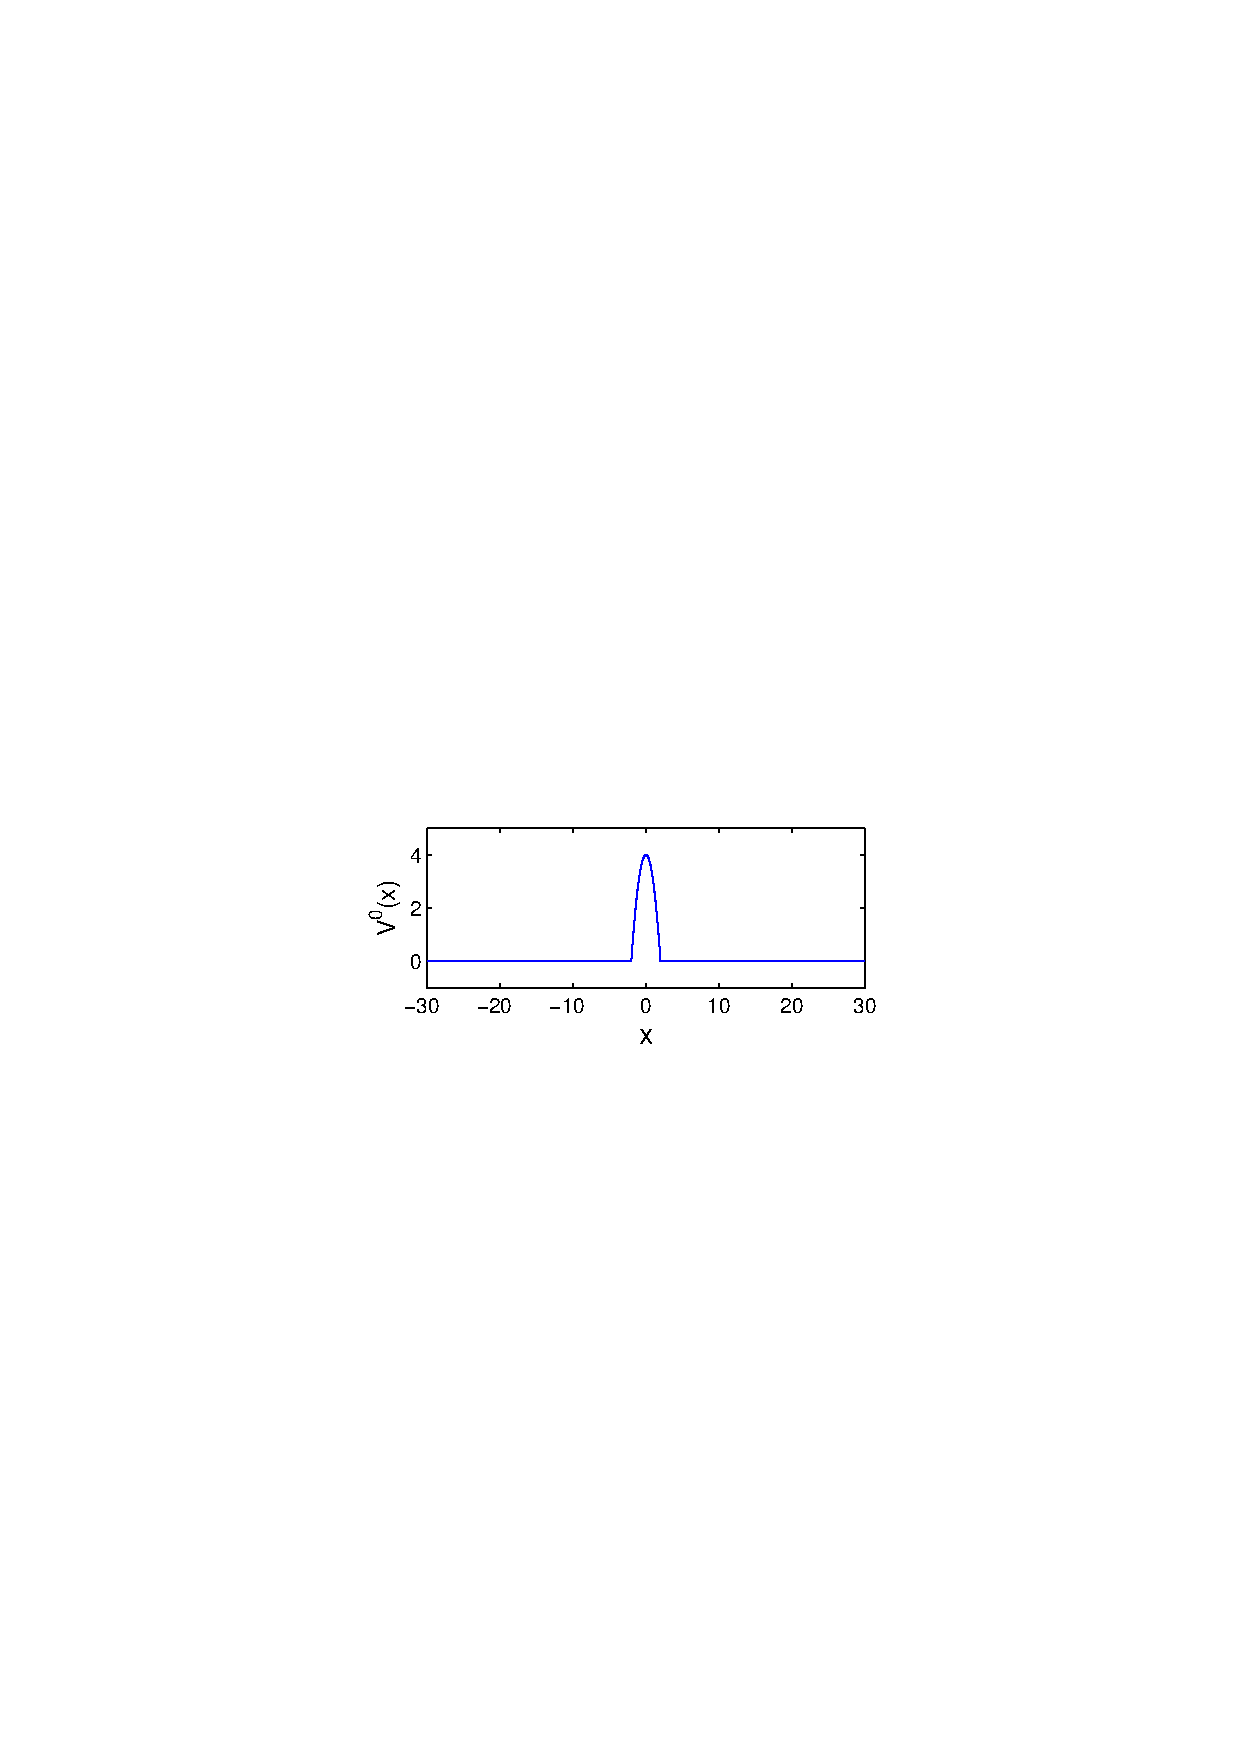
\includegraphics[width=0.4\textwidth]{Figures1/v1_mr.pdf}\\
\includegraphics[width=0.4\textwidth]{Figures1/v2_mr.pdf}\\
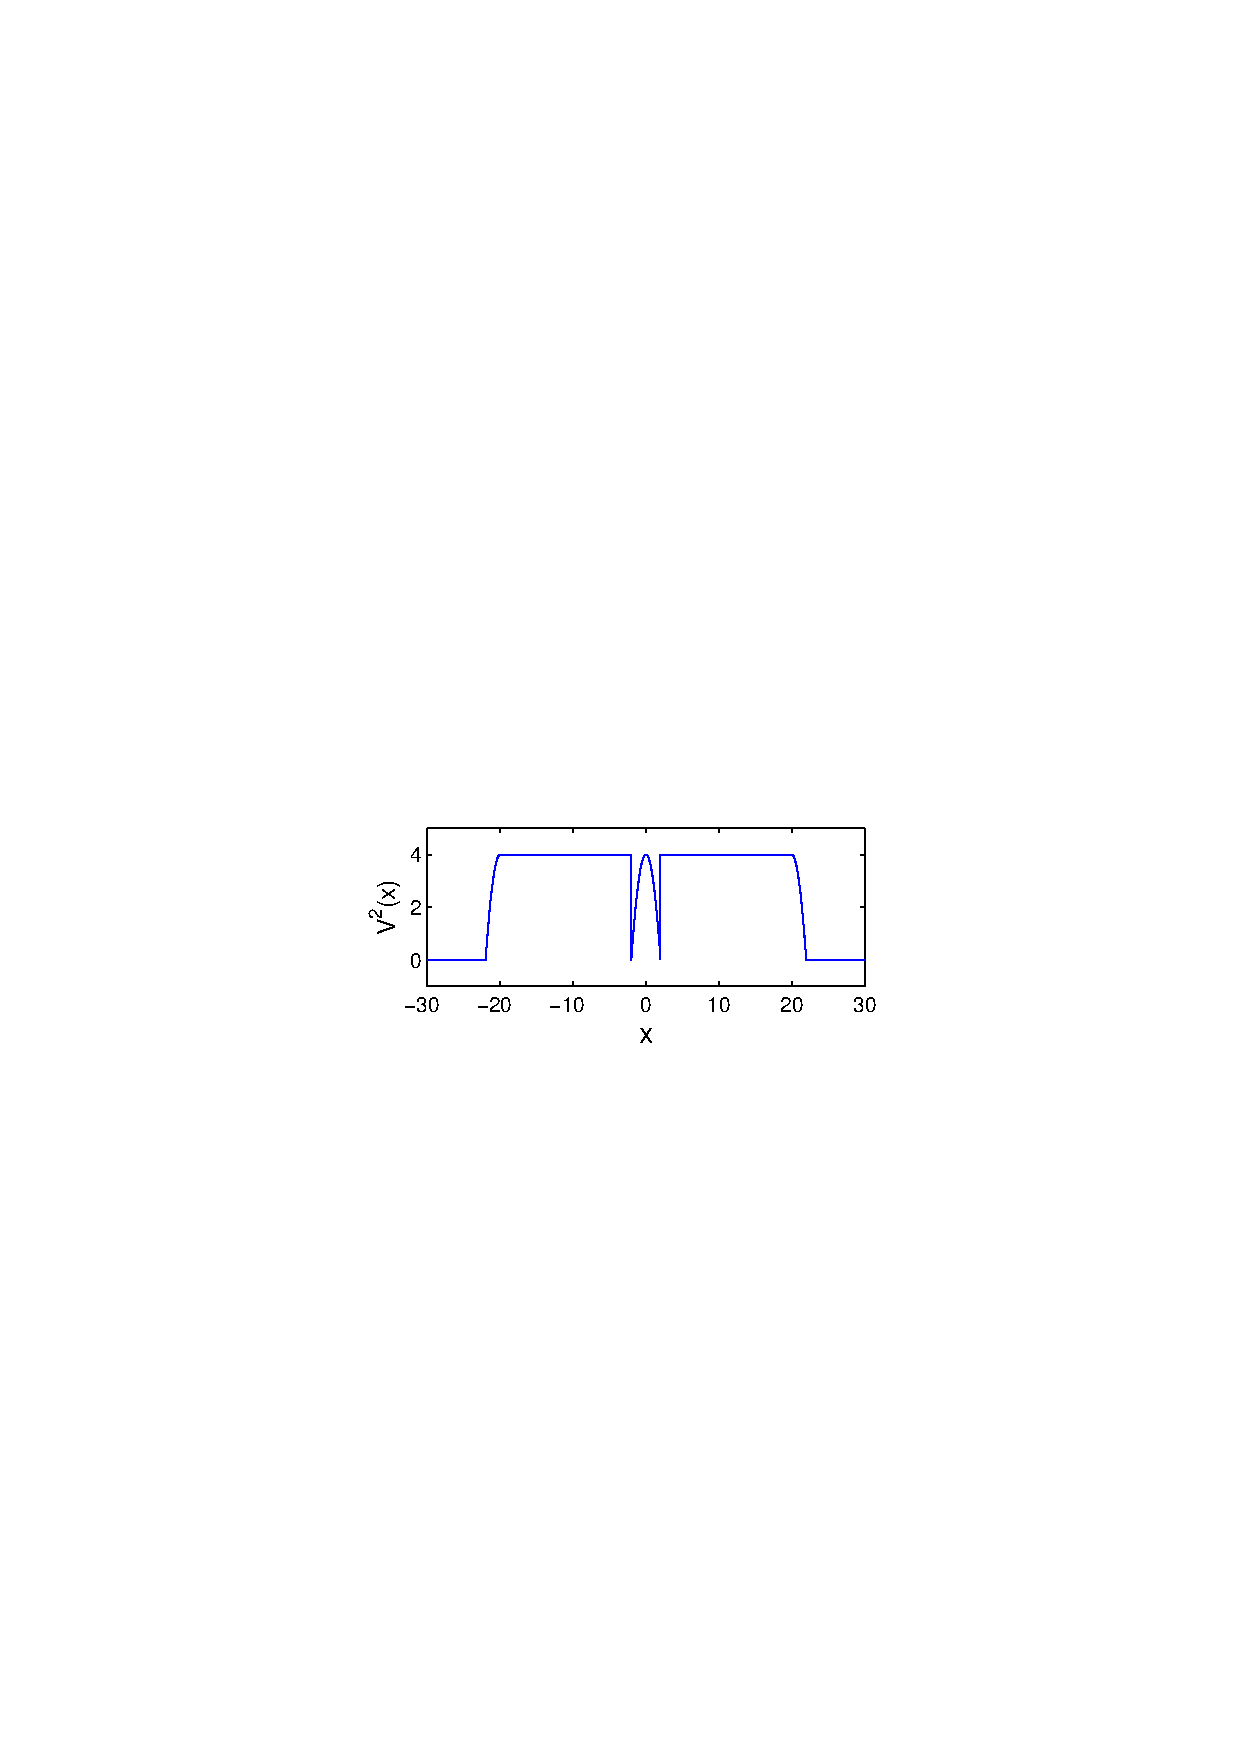
\includegraphics[width=0.4\textwidth]{Figures1/v3_mr.pdf}
\vspace{-2mm}
\caption{\footnotesize Optimal value functions $V^t$ (for $b =
\false$) for time horizons (i.e., decision stages remaining) $t=0$,
$t=1$, and $t=2$ on the \MarsRover\ problem.  For $x \in [-2,2]$, the
rover automatically takes a picture and receives a reward quadratic in
$x$.  For $V^1$, the rover may move up to 10 units in
either direction, reaching the full reward of $4$ up
to $x = \pm 10$ and non-zero reward up to $x = \pm 12$. 
For $V^2$, the rover can move up to 20 units in two time steps,
allowing it to achieve non-zero reward up to $x = \pm 12$.}
\label{fig:opt_graph}
%\vspace{-2mm}
\end{figure}
%%%%%%%%%%%%%%%%%%%%%%%%%%%%%%%%%%%%%%%%%%%%%%%%%%%%%%%%%%%%%%%%%%%%%%%%%%

%%%%%%%%%%%%%%%%%%%%%%%%%%%%%%%%%%%%%%%%%%%%%%%%%%%%%%%%%%%%%%%%%%%%%%%%%%
\begin{figure}[t!]
\centering
%\subfigure{
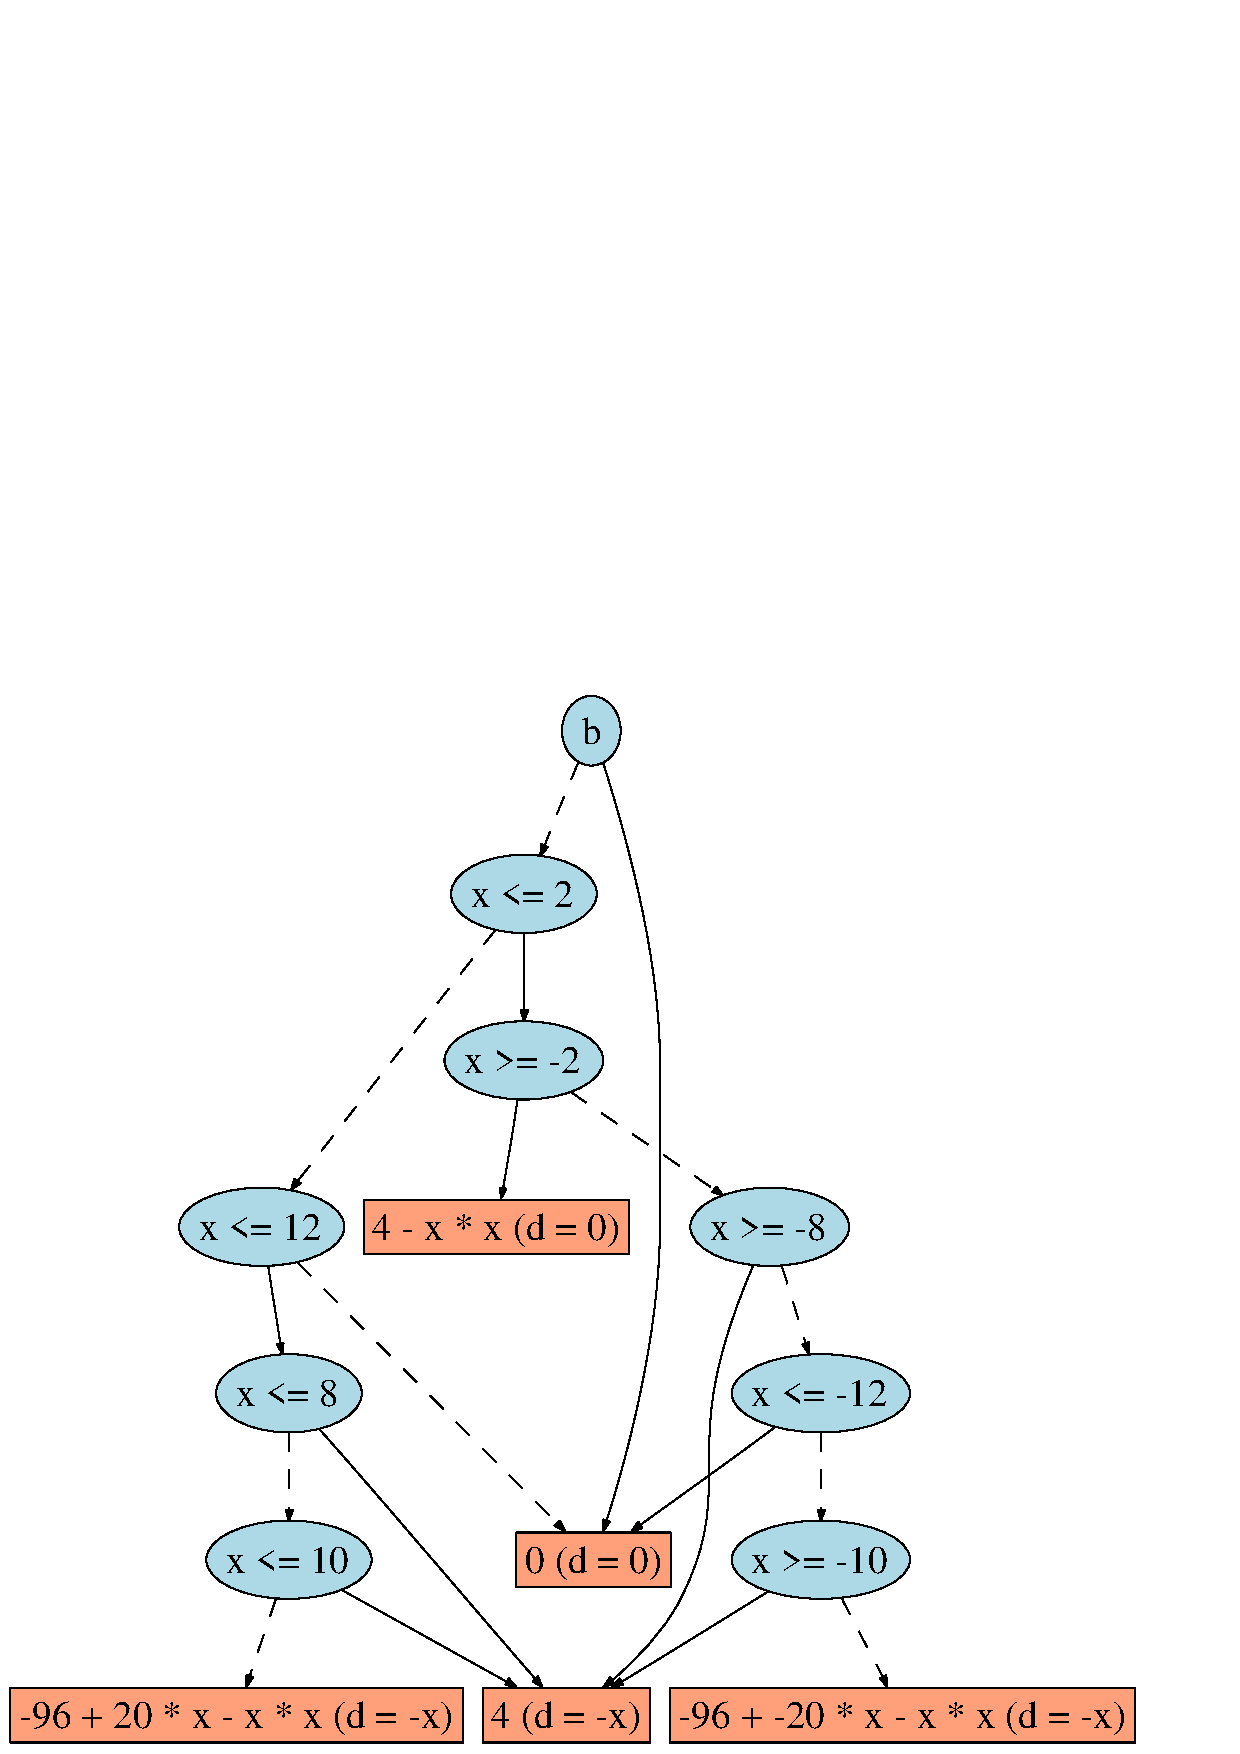
\includegraphics[width=0.5\textwidth]{Figures1/v2_mr_dd.pdf}
%\vspace{-3mm}
\caption{\footnotesize Optimal value function $V^1$ for the
\MarsRover\ problem represented as an extended algebraic decision
diagram (XADD).  Here the solid lines represent the $\true$ branch for
the decision and the dashed lines the $\false$ branch.  To evaluate
$V^1(x)$ for any state $x$, one simply traverses the diagram in a
decision-tree like fashion until a leaf is reached where the
expression provides the value.  The second expression in parentheses
in each leaf provides the optimal action \emph{policy} for $d$ as a
function of the state that allows one to obtain $V^1(x)$.  This
closed-form policy can be derived as a byproduct of symbolic dynamic
programming as we discuss later.}
\label{fig:opt_val_pol}
%\vspace{-3mm}
\end{figure}
%%%%%%%%%%%%%%%%%%%%%%%%%%%%%%%%%%%%%%%%%%%%%%%%%%%%%%%%%%%%%%%%%%%%%%%%%%

To get a sense of the form of the optimal solution to problems such as
the \MarsRover, we present the 0-, 1-, and 2-step time horizon solutions
for this problem in Figure~\ref{fig:opt_graph}; further, in symbolic form,
we display both the 1-step time horizon value function (the 2-step is
too large to display) and corresponding optimal policy in
Figure~\ref{fig:opt_val_pol}.  Here we see that the piecewise 
nature of the transition and reward function lead to
piecewise structure in the value function and policy.  And 
despite their striking simplicity, we are not aware of any exact
solution method to the above \MarsRover\ variant that can produce
such an optimal closed-form result.

To this end, we extend the symbolic dynamic programming (SDP) framework
of~\cite{sanner_uai11} to the case of continuous actions to obtain the
\emph{optimal closed-form} value function and policy for CSA-MDPs with
discrete noise, piecewise linear dynamics, and piecewise quadratic
rewards.  As the fundamental technical contribution of the paper, we
show how the \emph{continuous action maximization} step in the dynamic
programming backup can be evaluated optimally and symbolically and how
it can be efficiently realized in the extended algebraic decision diagram (XADD)
we use to perform all SDP operations.  This
allows us to obtain the \emph{first} algorithm to derive exact closed-form
solutions to this class of CSA-MDPs along with a closed-form
representation of the optimal policy
(cf. Figure~\ref{fig:opt_val_pol}).  
%- extension to XADDs
%- solutions for multivariate actions and quadratic reward
%- automatic derivation of the policy
%- first exact solution to variants of multi-inventory control
%  problem, water reservoir, and quadratic reward problems with
%  piecewise dynamics
We empirically evaluate the time and space required to compute exact
solutions to the \MarsRover\ problem for different time horizons, as
well as \WaterReservoir\ and multivariate action \InventoryControl\
studied in operations research showing the first exact solutions for
these problems can be practically computed for reasonable horizons.

\section{Continuous State and Action MDPs}

\label{sec:dcmdps}

We first introduce continuous state and action Markov decision
processes (CSA-MDPs) and then review their finite-horizon solution via
dynamic programming building on~\cite{sanner_uai11}.  

\subsection{Factored Representation}

In a CSA-MDP, states will be represented by vectors of variables
$(\vec{b},\vec{x}) = ( b_1,\ldots,b_n,x_{1},\ldots,x_m )$.  We assume
that each state variable $b_i$ ($1 \leq i \leq n$) is
boolean$\,$ s.t. $b_i \in \{ 0,1 \}$ and each $x_j$ ($1 \leq j \leq m$) is 
continuous s.t. $x_j \in [L_j,U_j]$ for $L_j,U_j \in
\mathbb{R}; L_j \leq U_j$.  We also assume a finite set of $p$ actions $A
= \{ a_1(\vec{y}_1), \ldots, a_p(\vec{y}_p) \}$, where the $\vec{y}$ denote
\emph{continuous action parameters} for the corresponding action.

A CSA-MDP is defined by the following: (1) a state transition model
$P(\vec{b}',\vec{x}'|\cdots,a,\vec{y})$, which specifies the probability of
the next state $(\vec{b}',\vec{x}')$ conditioned on a subset of the
previous and next state (defined below) and action $a$; (2) a reward
function $R(\vec{b},\vec{x},a,\vec{y})$, which specifies the immediate reward
obtained by taking action $a$ in state $(\vec{b},\vec{x})$; and (3) a
discount factor $\gamma, \; 0 \leq \gamma \leq 1$.\footnote{If time is
explicitly included as one of the continuous state variables, $\gamma
= 1$ is typically used, unless discounting by horizon (different from
the state variable time) is still intended.}  
A policy $\pi$
specifies the action $\pi(\vec{b},\vec{x})$ to take in each state
$(\vec{b},\vec{x})$.  Our goal is to find an optimal sequence of
horizon-dependent policies $\Pi^* = (\pi^{*,1},\ldots,\pi^{*,H})$
that maximizes the expected sum of discounted rewards over a horizon
$h \in H; H \geq 0$:\footnote{$H=\infty$ is allowed if an optimal policy has a
finitely bounded value (guaranteed if $\gamma < 1$); for $H=\infty$, 
the optimal policy is independent of horizon, 
i.e., $\forall h \geq 0, \pi^{*,h} = \pi^{*,h+1}$.}
\begin{align}
V^{\Pi^*}(\vec{x}) & = E_{\Pi^*} \left[ \sum_{h=0}^{H} \gamma^h \cdot r^h \Big| \vec{b}_0,\vec{x}_0 \right], \label{eq:vfun_def}
\end{align}
Here $r^h$ is the reward obtained at horizon $h$ following $\Pi^*$ where 
we assume starting state $(\vec{b}_0,\vec{x}_0)$ at $h=0$.
 
CSA-MDPs as defined above are naturally factored~\cite{boutilier99dt}
in terms of state variables $(\vec{b},\vec{x})$; as such transition
structure can be exploited in the form of a dynamic Bayes net
(DBN)~\cite{dbn} where the individual conditional probabilities
$P(b_i'|\cdots,a)$ and $P(x_j'|\cdots,a)$ condition on a subset of the
variables in the current and next state.  We disallow \emph{synchronic
arcs} (variables that condition on each other in the same time slice) 
within the binary $\vec{b}$ and continuous variables $\vec{x}$, 
but we allow synchronic arcs from $\vec{b}$ to $\vec{x}$ (note that
these conditions enforce the directed acyclic graph requirements of
DBNs).
%from variables in $\vec{b}$ to each other and to $\vec{x}$.
%variables to condition on binary
%them between  to enforce directed graph
%properties for \emph{synchronic arcs} among binary variables 
%, we assume a total ordering over
%binary and continuous variables and let $\vec{b}_{<i}$
%($\vec{x}_{<j}$) represent all variables lower than $b_i$ ($x_j$) in
%the ordering; furthermore we asssume and that all 
%$\vec{b}$ come before $\vec{x}$.  
We write the joint transition model as
\begin{align}
P(\vec{b}',&\vec{x}'|\vec{b},\vec{x},a,\vec{y}) = \label{eq:dbn} \\
& \prod_{i=1}^n P(b_i'|\vec{b},\vec{x},a,\vec{y}) \prod_{j=1}^m P(x_j'|\vec{b},\vec{b}',\vec{x},a,\vec{y}) \nonumber 
\end{align}
where $P(b_i'|\vec{b},\vec{x},a,\vec{y})$ may condition on a subset of
$\vec{b}$, $\vec{x}$, and $\vec{y}$ and likewise 
$P(x_j'|\vec{b},\vec{b}',\vec{x},a,\vec{y})$ may condition on a subset of
$\vec{b}$, $\vec{b}'$, $\vec{x}$, and $\vec{y}$.

We call the conditional probabilities
$P(b_i'|\vec{b},\vec{x},a,\vec{y})$ for \emph{binary} variables $b_i$
($1 \leq i \leq n$) conditional probability functions (CPFs) --- not
tabular enumerations, because in general these functions can condition
on both discrete and continuous state.  For the \emph{continuous}
variables $x_j$ ($1 \leq j \leq m$), we represent the CPFs
$P(x_j'|\vec{b},\vec{b'},\vec{x},a,\vec{y})$ with \emph{conditional
stochastic linear equations} (CSLEs).  For the solution provided here,
we only require three properties of these CSLEs: (1) they are
\emph{Markov}, meaning that they can only condition on the previous
state, (2) they are piecewise linear (pieces entering through the
conditional part) and (2) they are \emph{deterministic} meaning that
the next state must be uniquely determined from the previous state
(i.e., $x_1' = x_1 + x_2^2$ is deterministic whereas $x_1'^2 = x_1^2$
is not because $x_1' = \pm x_1$).\footnote{While the
\emph{deterministic} requirement may seem to conflict with the label
of \emph{stochastic}, we note that stochasticity enters through the
conditional component to be discussed in a moment.}  Otherwise, we
allow for arbitrary functions in these Markovian, conditional
deterministic equations as in the following example:
\vspace{-3mm}

{\footnotesize
\begin{align}
P(x_1' | \vec{b},\vec{b}',\vec{x},a) = \delta\left[ x_1' - 
\begin{cases}
b_1' \land x_2^2 \leq 1 : & \exp(x_1^2 - x_2^2) \\
\neg b_1' \lor  x_2^2 > 1 : & x_1 + x_2 \\
\end{cases}
\right] \label{eq:ex_csde}
\end{align}}
Here %the next-state of $x_1'$ is independent of the action $a$;
the use of the Dirac $\delta[\cdot]$ function ensures that this is a
conditional probability function that integrates to 1 over $x_1'$
in this case.  But in more intuitive terms, one can see that this
$\delta[\cdot]$ encodes the deterministic transition 
equation $x_1' = \ldots$ where $\ldots$ is the conditional portion 
of~\eqref{eq:ex_csde}.
In this work, we require all CSLEs in the transition
function for variable $x_i'$ to use the $\delta[\cdot]$ as shown in this
example.

It will be obvious that CSLEs in the form of \eqref{eq:ex_csde} are
\emph{conditional linear equations}; they are furthermore \emph{stochastic}
because they can condition on boolean random variables in the same time slice
that are stochastically sampled, e.g., $b_1'$ in
\eqref{eq:ex_csde}.  Of course, these CSLEs are restricted in that
they cannot represent general stochastic noise (e.g., Gaussian noise),
but we note that this representation effectively allows modeling of
continuous variable transitions as a mixture of $\delta$ functions,
which has been used heavily in previous exact continuous state MDP 
solutions~\cite{feng04,li05,hao09}.  

We allow 
the reward function $R_a(\vec{b},\vec{x})$
to be a piecewise quadratic function of the current state
for each action $a \in A$ with parameters $\vec{y}$, for example:
\begin{align}
R_a(\vec{b},\vec{x},\vec{y}) = \begin{cases}
x_1^2 + x_2^2 \leq 1 : & 1 - x_1^2 - x_2^2  \\
x_1^2 + x_2^2 > 1 : & 0 \\
\end{cases} \label{eq:simple_reward}
\end{align}
or even 
\begin{align}
R_a(\vec{b},\vec{x},\vec{y}) & = 10 x_3 x_4 \exp(x_1^2 + \sqrt{x_2}) \label{eq:expr_reward}
\end{align}

With our CSA-MDP now completely defined, our next objective
is to solve it.

\subsection{Solution Methods}

\label{sec:soln}

Now we provide a continuous state generalization of {\it
value iteration}~\cite{bellman}, which is a dynamic programming
algorithm for constructing optimal policies.  It proceeds by
constructing a series of $h$-stage-to-go value functions
$V^h(\vec{b},\vec{x})$.  Initializing $V^0(\vec{b},\vec{x})$ 
(e.g., to $V^0(\vec{b},\vec{x}) = 0$) 
we define the quality of taking action $a$ in state
$(\vec{b},\vec{x})$ and acting so as to obtain $V^{h}(\vec{b},\vec{x})$ 
thereafter as the following:
\vspace{-3mm}

{\footnotesize
\begin{align}
& Q_a^{h+1}(\vec{b},\vec{x}) = R_a(\vec{b},\vec{x}) + \gamma \cdot \label{eq:qfun} \\ 
& \sum_{\vec{b}'} \int_{\vec{x}'} \left( \prod_{i=1}^n P(b_i'|\vec{b},\vec{x},a) \prod_{j=1}^m P(x_j'|\vec{b},\vec{b}',\vec{x},a) \right) V^h(\vec{b}',\vec{x}') d\vec{x}' \nonumber
\end{align}}

Given $Q_a^h(\vec{b},\vec{x})$ for each $a \in A$, we can proceed
to define the $h+1$-stage-to-go value function as follows:
\begin{align}
V^{h+1}(\vec{b},\vec{x}) & = \max_{a \in A} \left\{ Q^{h+1}_a(\vec{b},\vec{x}) \right\} \label{eq:vfun}
\end{align}

If the horizon $H$ is finite, then the optimal value function is
obtained by computing $V^H(\vec{b},\vec{x})$ and the optimal
horizon-dependent policy $\pi^{*,h}$ at each stage $h$ can be easily
determined via 
$\pi^{*,h}(\vec{b},\vec{x}) = \argmax_a Q^h_a(\vec{b},\vec{x})$.  
If the horizon 
$H = \infty$ and the optimal policy has finitely bounded value, 
then value iteration can terminate at horizon $h+1$ if 
$V^{h+1} = V^{h}$; then 
$\pi^*(\vec{b},\vec{x}) = \argmax_a Q^{h+1}_a(\vec{b},\vec{x})$.

Of course this is simply the \emph{mathematical} definition.  In the
discrete-only case, we can always compute this in tabular form;
however, how to compute this for DC-MDPs with reward and transition
function as previously defined is the objective of the symbolic
dynamic programming algorithm that we define next.

\section{Symbolic Dynamic Programming}

As it's name suggests, symbolic dynamic programming (SDP)~\cite{fomdp}
is simply the process of performing dynamic programming (in this case
value iteration) via symbolic manipulation.  While SDP as defined
in~\cite{fomdp} was previously only used with piecewise
constant functions, we now generalize the representation to work with
general piecewise functions needed for DC-MDPs in this paper.  

Before we define our solution, however, we must formally define our
case representation and symbolic case operators.

\subsection{Case Representation and Operators}

Throughout this paper, we will assume that all symbolic functions
can be represented in \emph{case} form as follows:
{%\footnotesize 
\begin{align*}
f = 
\begin{cases}
  \phi_1: & f_1 \\ 
 \vdots&\vdots\\ 
  \phi_k: & f_k \\ 
\end{cases}
\end{align*}
}
Here the $\phi_i$ are logical formulae defined over the state
$(\vec{b},\vec{x})$ that can include arbitrary logical ($\land,\lor,\neg$)
combinations of (a) boolean variables in $\vec{b}$ and (b) 
inequalities ($\geq,>,\leq,<$), equalities ($=$), or disequalities ($\neq$)
where the left and right operands can be \emph{any} function of one or more 
variables in $\vec{x}$.  
Each $\phi_i$ will be disjoint from the other $\phi_j$ ($j \neq i$); 
however the $\phi_i$ may not exhaustively cover the state space, hence
$f$ may only be a \emph{partial function} and may be undefined for some
state assignments.
%\footnote{In the context of SDP, states whose value
%at horizon $h$ is undefined correspond to states that cannot reach any
%defined state of the reward in horizon $h$.}
The $f_i$ can be \emph{any} functions of the state
variables in $\vec{x}$.  

As concrete examples, consider the transition representation for
KNAPSACKin Ex.~\ref{ex:knapsack}, the optimal value function for
KNAPSACKfrom~\eqref{eq:vfun_knapsack}, or any of
\eqref{eq:ex_csde}, \eqref{eq:simple_reward}, or \eqref{eq:expr_reward}.

\emph{Unary operations} such as scalar multiplication $c\cdot f$ (for
some constant $c \in \mathbb{R}$) or negation $-f$ on case statements
$f$ are straightforward; the unary operation is simply applied to each
$f_i$ ($1 \leq i \leq k$). Intuitively, to perform a \emph{binary
  operation} on two case statements, we simply take the cross-product
of the logical partitions of each case statement and perform the
corresponding operation on the resulting paired partitions.  Letting
each $\phi_i$ and $\psi_j$ denote generic first-order formulae, we can
perform the ``cross-sum'' $\oplus$ of two (unnamed) cases in the
following manner:

{\footnotesize 
\begin{center}
\begin{tabular}{r c c c l}
&
\hspace{-6mm} 
  $\begin{cases}
    \phi_1: & f_1 \\ 
    \phi_2: & f_2 \\ 
  \end{cases}$
$\oplus$
&
\hspace{-4mm}
  $\begin{cases}
    \psi_1: & g_1 \\ 
    \psi_2: & g_2 \\ 
  \end{cases}$
&
\hspace{-2mm} 
$ = $
&
\hspace{-2mm}
  $\begin{cases}
  \phi_1 \wedge \psi_1: & f_1 + g_1 \\ 
  \phi_1 \wedge \psi_2: & f_1 + g_2 \\ 
  \phi_2 \wedge \psi_1: & f_2 + g_1 \\ 
  \phi_2 \wedge \psi_2: & f_2 + g_2 \\ 
  \end{cases}$
\end{tabular}
\end{center}
}
\normalsize

Likewise, we can perform $\ominus$ and $\otimes$ by,
respectively, subtracting or multiplying partition values (as opposed
to adding them) to obtain the result.  Some partitions resulting from
the application of the $\oplus$, $\ominus$, and $\otimes$ operators
may be inconsistent (infeasible); we may simply discard such 
partitions as they are irrelevant to the function value.

For SDP, we'll also need to perform maximization, restriction,
and substitution on case statements.  
\emph{Symbolic maximization} is fairly straightforward
to define:
\vspace{-5mm}

{\footnotesize
\begin{center}
\begin{tabular}{r c c c l}
&
\hspace{-9mm} $\max \Bigg(
  \begin{cases}
    \phi_1: & f_1 \\ 
    \phi_2: & f_2 \\ 
  \end{cases}$
$,$
&
\hspace{-4mm}
  $\begin{cases}
    \psi_1: & g_1 \\ 
    \psi_2: & g_2 \\ 
  \end{cases} \Bigg)$
&
\hspace{-4mm} 
$ = $
&
\hspace{-4mm}
  $\begin{cases}
  \phi_1 \wedge \psi_1 \wedge f_1 > g_1    : & f_1 \\ 
  \phi_1 \wedge \psi_1 \wedge f_1 \leq g_1 : & g_1 \\ 
  \phi_1 \wedge \psi_2 \wedge f_1 > g_2    : & f_1 \\ 
  \phi_1 \wedge \psi_2 \wedge f_1 \leq g_2 : & g_2 \\ 
  \phi_2 \wedge \psi_1 \wedge f_2 > g_1    : & f_2 \\ 
  \phi_2 \wedge \psi_1 \wedge f_2 \leq g_1 : & g_1 \\ 
  \phi_2 \wedge \psi_2 \wedge f_2 > g_2    : & f_2 \\ 
  \phi_2 \wedge \psi_2 \wedge f_2 \leq g_2 : & g_2 \\ 
  \end{cases}$
\end{tabular}
\end{center}
}
One can verify that the resulting case statement is still
within the case language defined previously.  At first
glance this may seem like a cheat and little is gained
by this symbolic sleight of hand.  However, simply
having a case partition representation that is closed under 
maximization will facilitate the closed-form regression 
step that we need for SDP.\ \  Furthermore, the 
XADD that we introduce later will be able to exploit the 
internal decision structure of this
maximization to represent it much more compactly.

The next operation of \emph{restriction} is fairly simple: in this
operation, we want to restrict a function $f$ to apply only in cases
that satisfy some formula $\phi$, which we write as $f|_{\phi}$.  
This can be done by simply appending $\phi$ to each case partition
as follows:
{\footnotesize
\begin{center}
\begin{tabular}{r c c l}
&
\hspace{-6mm} 
  $f = \begin{cases}
    \phi_1: & f_1 \\ 
   \vdots&\vdots\\ 
    \phi_k: & f_k \\ 
  \end{cases}$
&

&
\hspace{-2mm}
  $f|_{\phi} = \begin{cases}
    \phi_1 \land \phi : & f_1 \\ 
   \vdots&\vdots\\ 
    \phi_k \land \phi : & f_k \\ 
  \end{cases}$
\end{tabular}
\end{center}
}
Clearly $f|_{\phi}$ only applies when $\phi$ holds and is
undefined otherwise, hence $f|_{\phi}$ is a partial function
unless $\phi \equiv \top$.

The final operation that we need to define for case
statements is substitution.  \emph{Symbolic substitution} simply takes
a set $\sigma$ of variables and their substitutions, e.g., 
$\sigma = \{ x_1' / (x_1 \hspace{-.8mm} + \hspace{-.8mm} x_2), x_2' / x_1^2 \hspace{-.3mm} \exp(x_2) \}$ where
the LHS of the $/$ represents the substitution variable and the
RHS of the $/$ represents 
the expression that should be substituted in its place.  No variable
occurring in any RHS expression of $\sigma$ can also occur in any 
LHS expression of $\sigma$.
We write the substitution of a non-case function $f_i$ with $\sigma$ 
as $f_i\sigma$; as an example, for the $\sigma$ defined previously and 
$f_i = x_1' + x_2'$ then $f_i\sigma = x_1 + x_2 + x_1^2 \exp(x_2)$ as
would be expected.  We can also substitute into case partitions $\phi_j$
by applying $\sigma$ to each inequality operand; as an example, if
$\phi_j \equiv x_1' \leq \exp(x_2')$ then 
$\phi_j \sigma \equiv x_1 + x_2 \leq \exp(x_1^2 \exp(x_2))$.
Having now defined substitution of $\sigma$ for non-case functions $f_i$ and case
partitions $\phi_j$ we can define it for case statements in general:

{\footnotesize
\begin{center}
\begin{tabular}{r c c l}
&
\hspace{-6mm} 
  $f = \begin{cases}
    \phi_1: & f_1 \\ 
   \vdots&\vdots\\ 
    \phi_k: & f_k \\ 
  \end{cases}$
&

&
\hspace{-2mm}
  $f\sigma = \begin{cases}
    \phi_1\sigma: & f_1\sigma \\ 
   \vdots&\vdots\\ 
    \phi_k\sigma: & f_k\sigma \\ 
  \end{cases}$
\end{tabular}
\end{center}
}
\normalsize

One property of substitution is that
if $f$ has mutually exclusive partitions $\phi_i$ ($1 \leq i \leq k$)
then $f\sigma$ must also have mutually exclusive partitions ---
this follows from the logical consequence that 
if $\phi_1 \land \phi_2 \models \bot$
then $\phi_1\sigma \land \phi_2\sigma \models \bot$.
%We will exploit this property next in SDP for DC-MDPs.

%%zz: entire subsection
\subsection{Maximization of continuous actions}


In the previous section, we covered the operations required for the SDP algorithm. Here we address the issue of maximizing a function (e.g., Q-function) over continuous action variables.

To compute the maximum of any arbitrary function $f$ in the case format, over the continuous variable $d$, we maintain a closed-form case representation. Using the mutually exclusive and disjoint property of partitions, :\footnote{Any case partition without this property can be converted into its equivalent case representation using logical operators such as $\wedge$ and $\neg$} we claim that the following equality holds: 
\begin{equation}
\sum_{d}\max_{i}\varphi_{i}f_{i}=\max_{i}\max_{d}\varphi_{i}f_{i}
\end{equation}

Since we care about taking the maximum of each partition and obtaining an overall maximum for the function and the partitions have no junctions, the above holds for our case representation. Thus we compute the maximum separately for each case partition and then $\max$ over the final results. The final maximum is a symbolic maximum as explained before, the inside maximum for each partition is the operation defined here. 

To continue with maximization in one partition, we use our \MarsRoverNL example in one of the branches of the first iteration for continuous maximization that covers this technique completely. This branch is obtained from replacing the transition function of each variable in the reward function for the conditions $ \neg b\wedge (x\geq 2)\wedge (d\leq 10) \wedge (d\geq -10)\wedge  (x+d\leq 2) \wedge (x+d\geq -2) $ to obtain the root value of $ 4 - (x+a)^2 $.

We also consider some mathematical definitions for the technique of maximizing the continuous action: 
\begin{enumerate}
\item A real-valued function f defined on the real domain is said to have a global (or absolute) maximum point at the point x, if for all x :$ f(x^{*}) \geq f(x) $. The value of the function at this point is the maximum of the function.
\item By Fermat's theorem, the local maxima (and minima) of a function can occur only at its critical points where either the function is not differentiable or its derivative is 0 at that point. 
\item Boundedness theorem states that a continuous function f in the closed interval (a,b) is bounded on that interval. That is, there exist real numbers m and M such that:
\begin{align*}
\forall x \in \{a,b\} : m \leq f(x) \leq M 
\end{align*}
\end{enumerate}

Based on these definitions, the maximum value of a function is defined at the boundaries and roots of that function according to the continuous variable $d$. If this function were linear and a polynomial of a certain degree k, then the maximum for that function would occur on any of the (k-1) roots of the function or at the lower and upper bounds defined for it.
\\We can write the explicit functions for these bounds in  \emph{piecewise linear case form} for the respective lower and upper bounds $LB$, $UB$ and possible roots of our example as shown below. The maximum of all the lower bounds is obtained by taking a maximum over this set and the maximum of the upper bounds is obtained by taking a minimum over the set of UB.

{\footnotesize
\begin{center}
\begin{tabular}{r c c c l}
&
\hspace{-9mm} $LB:= \max
  \begin{cases}
d \geq -10 \\ 
d \geq -2 -x\\ 
  \end{cases}$
$=$
&
\hspace{-4mm}
$  \begin{cases}
x \leq 8: & -2 -x \\ 
x \geq 8: &-10\\ 
  \end{cases}$
&
\hspace{-4mm} 
\\
&
\hspace{-4mm}
$UB:= \max
  \begin{cases}
d \leq 10 \\ 
d \leq 2 -x\\ 
  \end{cases}$
$=$
&
\hspace{-4mm}
$  \begin{cases}
x \geq -8: & 2 -x \\ 
x \leq -8: &10\\ 
  \end{cases}$
&
\hspace{-4mm} 
\\
&
\hspace{-4mm}
$Roots:= 
  \begin{cases}
-2\cdot x -2 \cdot d=0  := -x \\ 

  \end{cases}$
\end{tabular}
\end{center}
}

A lower bound on action $d$ occurs when the inequalities of $\geq ,>$ have action $d$ on their LHS; then any expression on the RHS is considered a lower bound on action $d$. Similar to this, an upper bound occurs for inequalities of $\leq , <$ and the RHS expression is considered an upper bound for action $d$. 
The roots of the function are also defined by taking the first derivative of $f$ with respect to $d$ and setting it to zero.

To enforce correctness of bounds symbolically we must have $LB \leq Roots \leq UB$, so we add the pair of constraints for the bounds to the root constraint:

{\footnotesize
\begin{center}
\begin{tabular}{r c c c l}
&
\hspace{-9mm} $
  \begin{cases}
-10 \leq -x \\ 
-2 -x \leq -x \\ 
-x \leq 10 \\ 
-x \leq 2 -x\\ 
  \end{cases}$
$=$
&
\hspace{-4mm}
$ \begin{cases}
x \leq 10 \\ 
x \geq -10\\ 
  \end{cases}$
\end{tabular}
\end{center}
}
The other two statements can be removed as a tautology, to leave the final root partition as: 

\begin{align*}Roots:= 
 \begin{cases}
x \leq 10 \wedge x \geq -10:              & -x\\ 
\neg (x \leq 10 \wedge x \geq -10):    & 0\\ 
  \end{cases}
\end{align*}

Having the UB,LB and root of each case partition, we can maximize the value of each case function according to the bounds. We want to factor out the action variable $d$ (we show later that this is equal to maximizing the Q-function values in order to obtain the value function). This means replacing the continuous action with the possible maximum points; LB, UB and roots. Replacing the action with a constant, variable or another function is equal to applying the \emph{substitute} operator. Each substitution forms a partition of the final maximization over the three posibble maximum points: 

\begin{align*}
\max_{d}
\begin{cases}
4 - (x+ UB)^2 \\ 
4- (x+LB)^2 \\ 
4 - (x+Roots)^2\\ 
  \end{cases}
\end{align*}

We take the maximum of the UB and LB  substitutions and then maximum the result with the root substitution. Below shows the substituted maximum points:

{\footnotesize
\begin{center}
\begin{tabular} {r c c c l}
\hspace{-4mm}
$
\begin{cases}
x \leq -8 : & -96 + 20 \cdot x - x^2 \\ 
x \geq -8 : & 0 \\ 
\end{cases} $

\\
\hspace{-4mm}
$ \begin{cases}
x \leq 8 : & 0 \\ 
x \geq 8: & -96 -x^2 -20\cdot x\\
\end{cases}$
\hspace{-4mm} 
\\
\hspace{-4mm}
$\begin{cases}
x \leq 10 \wedge x \geq -10 : & 4 \\ 
x \leq 10 \wedge x \geq -10 : & 4 \\ 
\end{cases})$
\end{tabular}
\end{center}
}

The main partitions after the maximization over action $d$ is as below, the rest of the partitions hold the value of zero: 
\begin{align*}
\max_{d}
\begin{cases}
-10 \leq x \leq 10 : 4 \\ 
10 \leq x \leq 12  \wedge  -96-x^2-20\cdot x \geq 0: \\ -96-x^2-20\cdot x \geq 0 \\ 
-12 \leq x \leq -10  \wedge  -96-x^2+20\cdot x \geq 0:\\ -96-x^2+20\cdot x \geq 0 \\
  \end{cases}
\end{align*}

After taking the symbolic maximum over the partitions above, we also add all the constraints that did not effect the $d$ boundaries (i.e, $x\leq 2:false $ and $b:false$) which means only considering the partition values for $x \geq 2$ which takes out the final branch of the case partition above. 

%% end of maximization subsection

\subsection{Symbolic Dynamic Programming (SDP)}

% \ref{sec:dcmdps} \ref{sec:soln} \ref{eq:qfun} \ref{eq:vfun} 

In the SDP solution for DC-MDPs, our objective will be to take
a DC-MDP as defined in Section~\ref{sec:dcmdps}, apply value
iteration as defined in Section~\ref{sec:soln}, and produce
the final value optimal function $V^h$ at horizon $h$ in the form
of a case statement.

For the base case of $h=0$, we note that setting $V^0(\vec{b},\vec{x}) = 0$
(or to the reward case statement, if not action dependent)
%and $R(\vec{b},\vec{x})$ as described in Section~\ref{sec:dcmdps}
is trivially in the form of a case statement.  

Next, $h > 0$ requires the application of SDP.  
Fortunately, given our previously defined
operations, SDP is straightforward and can be divided into four 
steps: 
\begin{enumerate}
\item {\it Prime the Value Function}: Since $V^{h}$ will become
the ``next state'' in value iteration, we setup a substitution
$\sigma = \{ b_1 / b_1', \ldots, b_n / b_n', x_1 / x_1', \ldots, x_m / x_m' \}$
and obtain $V'^{h} = V^{h}\sigma$.
%where $V'^{h}$ is over $(\vec{b}',\vec{x}')$.

\item {\it Continuous Integration}: Now that we have our primed value
function $V'^{h}$ in case statement format defined over next state
variables $(\vec{b}',\vec{x}')$, we first evaluate the integral
marginalization $\int_{\vec{x}'}$ over the continuous variables
in~\eqref{eq:qfun}.  Because the lower and upper integration bounds
are respectively $-\infty$ and $\infty$
and we have
disallowed synchronic arcs between variables in $\vec{x}'$ 
in the transition DBN, we can marginalize out each
$x_j'$ independently, and in any order.  Using 
\emph{variable elimination}~\cite{varelim}, when marginalizing
over $x_j'$ we can factor out any functions independent of $x_j'$ --- 
that is, for $\int_{x_j'}$ in~\eqref{eq:qfun}, 
one can see that initially, 
the only functions that can include $x_j'$ are $V'^{h}$
and $P(x_j'|\vec{b},\vec{b}',\vec{x},a,\vec{y}) = \delta[x_j' - g(\vec{x})]$; 
hence, the first marginal over $x_j'$ need only be computed over
$\delta[x_j' - g(\vec{x})] V'^{h}$.

What follows is one of the \emph{key novel insights of SDP} in the context of
DC-MDPs --- the integration 
$\int_{x_j'} \delta[x_j' - g(\vec{x})] V'^{h} dx_j'$ 
simply \emph{triggers the substitution} $\sigma = \{ x_j' / g(\vec{x}) \}$
on $V'^{h}$, that is
\begin{align}
\int_{x_j'} \delta[x_j' - g(\vec{x})] V'^{h} dx_j' \; = \; V'^{h} \{x_j' / g(\vec{x}) \} . \label{eq:one_int}
\end{align}
Thus we can perform the
operation in~\eqref{eq:one_int} repeatedly in sequence \emph{for each}
$x_j'$ ($1 \leq j \leq m$) for every action $a$.  The only
additional complication is that the form of 
$P(x_j'|\vec{b},\vec{x},a,\vec{y})$ is a \emph{conditional} 
equation, c.f.~\eqref{eq:ex_csde}, and represented generically
as follows:
\begin{align}
   P(x_j'|\vec{b},\vec{x},a,\vec{y}) = \delta\left[ x_j' = \begin{cases}
    \phi_1: & f_1 \\ 
   \vdots&\vdots\\ 
    \phi_k: & f_k \\ 
  \end{cases} \right] \label{eq:cond_sub}
\end{align}
Hence to perform~\eqref{eq:one_int} on this more general
representation, we obtain that $\int_{x_j'} P(x_j'|\vec{b},\vec{x},a,\vec{y}) V'^{h} dx_j'$
\begin{align*}
    = \begin{cases}
    \phi_1: & V'^{h} \{ x_j' = f_1 \} \\ 
   \vdots&\vdots\\ 
    \phi_k: & V'^{h} \{ x_j' = f_k \}  \\ 
  \end{cases}
\end{align*}
In effect, we can read~\eqref{eq:cond_sub} as a \emph{conditional
substitution}, i.e., in each of the different \emph{previous state}
conditions $\phi_i$ ($1 \leq i \leq k$), we obtain a different
substitution for $x_j'$ appearing in $V'^{h}$ (i.e., $\sigma = \{ x_j' / f_i
\}$).  Here we note that because $V'^{h}$ is \emph{already} a case
statement, we can simply replace the single partition $\phi_i$ with the
multiple partitions of $V'^h \{ x_j' / f_i \}|_{\phi_i}$.\footnote{If $V'^h$
had mutually disjoint partitions then we note the restriction and
substitution operations preserve this disjointness.}  This reduces
the \emph{nested} case statement back down to a non-nested case
statement as in the following example:
\begin{align*}
    \begin{cases}
      \phi_1: & 
        \begin{cases}
          \psi_1: & f_{11} \\ 
          \psi_2: & f_{12}  \\ 
        \end{cases} \\
      \phi_2: & 
        \begin{cases}
          \psi_1: & f_{21} \\ 
          \psi_2: & f_{22}  \\ 
        \end{cases} \\
    \end{cases} & \; = \;
        \begin{cases}
          \phi_1 \land \psi_1: & f_{11} \\ 
          \phi_1 \land \psi_2: & f_{12}  \\ 
          \phi_2 \land \psi_1: & f_{21} \\ 
          \phi_2 \land \psi_2: & f_{22}  \\ 
        \end{cases} 
\end{align*}

To perform the full continuous integration, 
if we initialize 
$\tilde{Q}_a^{h+1} := V'^{h}$ for each action $a \in A$, and repeat
the above integrals for all $x_j'$, updating $\tilde{Q}_a^{h+1}$ each time,
then after elimination of all $x_j'$ ($1 \leq j \leq m$), we will have 
the partial regression of $V'^{h}$ for the continuous variables for
each action $a$ denoted by $\tilde{Q}_a^{h+1}$.
\item {\it Discrete Marginalization}: Now that we have our partial
regression $\tilde{Q}_a^{h+1}$ for each action $a$, we proceed
to derive the full backup $Q_a^{h+1}$ from $\tilde{Q}_a^{h+1}$
by evaluating the discrete 
marginalization $\sum_{\vec{b}'}$ in~\eqref{eq:qfun}.
Because we previously disallowed synchronic arcs
between the variables in $\vec{b}'$ 
in the transition DBN, we can sum out each variable $b_i'$ ($1 \leq i \leq n$) 
independently.  Hence, initializing
$Q_a^{h+1} := \tilde{Q}_a^{h+1}$
we perform the discrete regression by applying the following iterative
process \emph{for each} $b_i'$ in any order
for each action $a$:
\begin{align}
Q_a^{h+1} := & \left[ Q_a^{h+1} \otimes P(b_i'|\vec{b},\vec{x},a,\vec{y}) \right]|_{b_i' = 1} \nonumber \\
 & \oplus \left[ Q_a^{h+1} \otimes P(b_i'|\vec{b},\vec{x},a,\vec{y}) \right]|_{b_i' = 0}.
\end{align}
This requires a variant of the earlier restriction operator $|_v$ that
actually \emph{sets} the variable $v$ to the given value if present.
Note that both $Q_a^{h+1}$ and $P(b_i'|\vec{b},\vec{x},a,\vec{y})$ can be represented
as case statements (discrete CPTs \emph{are} case statements), 
and each operation produces a case statement.
Thus, once this process is complete, we have marginalized over
all $\vec{b}'$ and $Q_a^{h+1}$ is the symbolic representation
of the intended Q-function.
\item {it Continuous Maximization} Now that we have $Q_a^{h+1}$ in
the case format we perform continuous maximization for the continuous parameter $y$ as explained in the previous section. This step factors out the continuous action variable from the Q-function. 
\item {\it Maximization}: Now that we have $Q_a^{h+1}$ in
case format for each action $a \in \{a_1,\ldots,a_p\}$, obtaining
$V^{h+1}$ in case format as defined in~\eqref{eq:vfun} requires
sequentially applying
\emph{symbolic maximization} as defined previously:
\begin{align*}
V^{h+1} & = 
\max(Q_{a_1}^{h+1},\max(\ldots,\max(Q_{a_{p-1}}^{h+1},Q_{a_p}^{h+1})))
\end{align*}
\end{enumerate}
By induction, because $V^0$ is a case statement and applying
SDP to $V^h$ in case statement form produces $V^{h+1}$ in case
statement form, we have achieved our intended
objective with SDP.  On the issue of correctness,
we note that each operation above simply implements one of the
dynamic programming operations in \eqref{eq:qfun} or \eqref{eq:vfun}, 
so correctness simply follows from verifying (a) that each case
operation produces the correct result and that (b) each case operation
is applied in the correct sequence as defined in \eqref{eq:qfun} or 
\eqref{eq:vfun}.  

%To make this concrete, we provide an example of SDP for \Knapsack.

On a final note, we observe that SDP holds for \emph{any} symbolic
case statements; we have not restricted ourselves to rectangular
piecewise functions, piecewise linear functions, or even piecewise
polynomial functions.  As the SDP solution is purely symbolic,
SDP applies to \emph{any} DC-MDPs using bounded symbolic function 
that can be written in case format!  Of course, that is the theory,
next we meet practice.


%%%%%%%%%%%%%%%%%%%%%%%%%%%%%%%%%%%%%%%%%%%%%%%%%%%%%%%%%%%%%%%%%%%%%%%%%%
% V2 for marsrover
\begin{figure*}[t]
\begin{center}
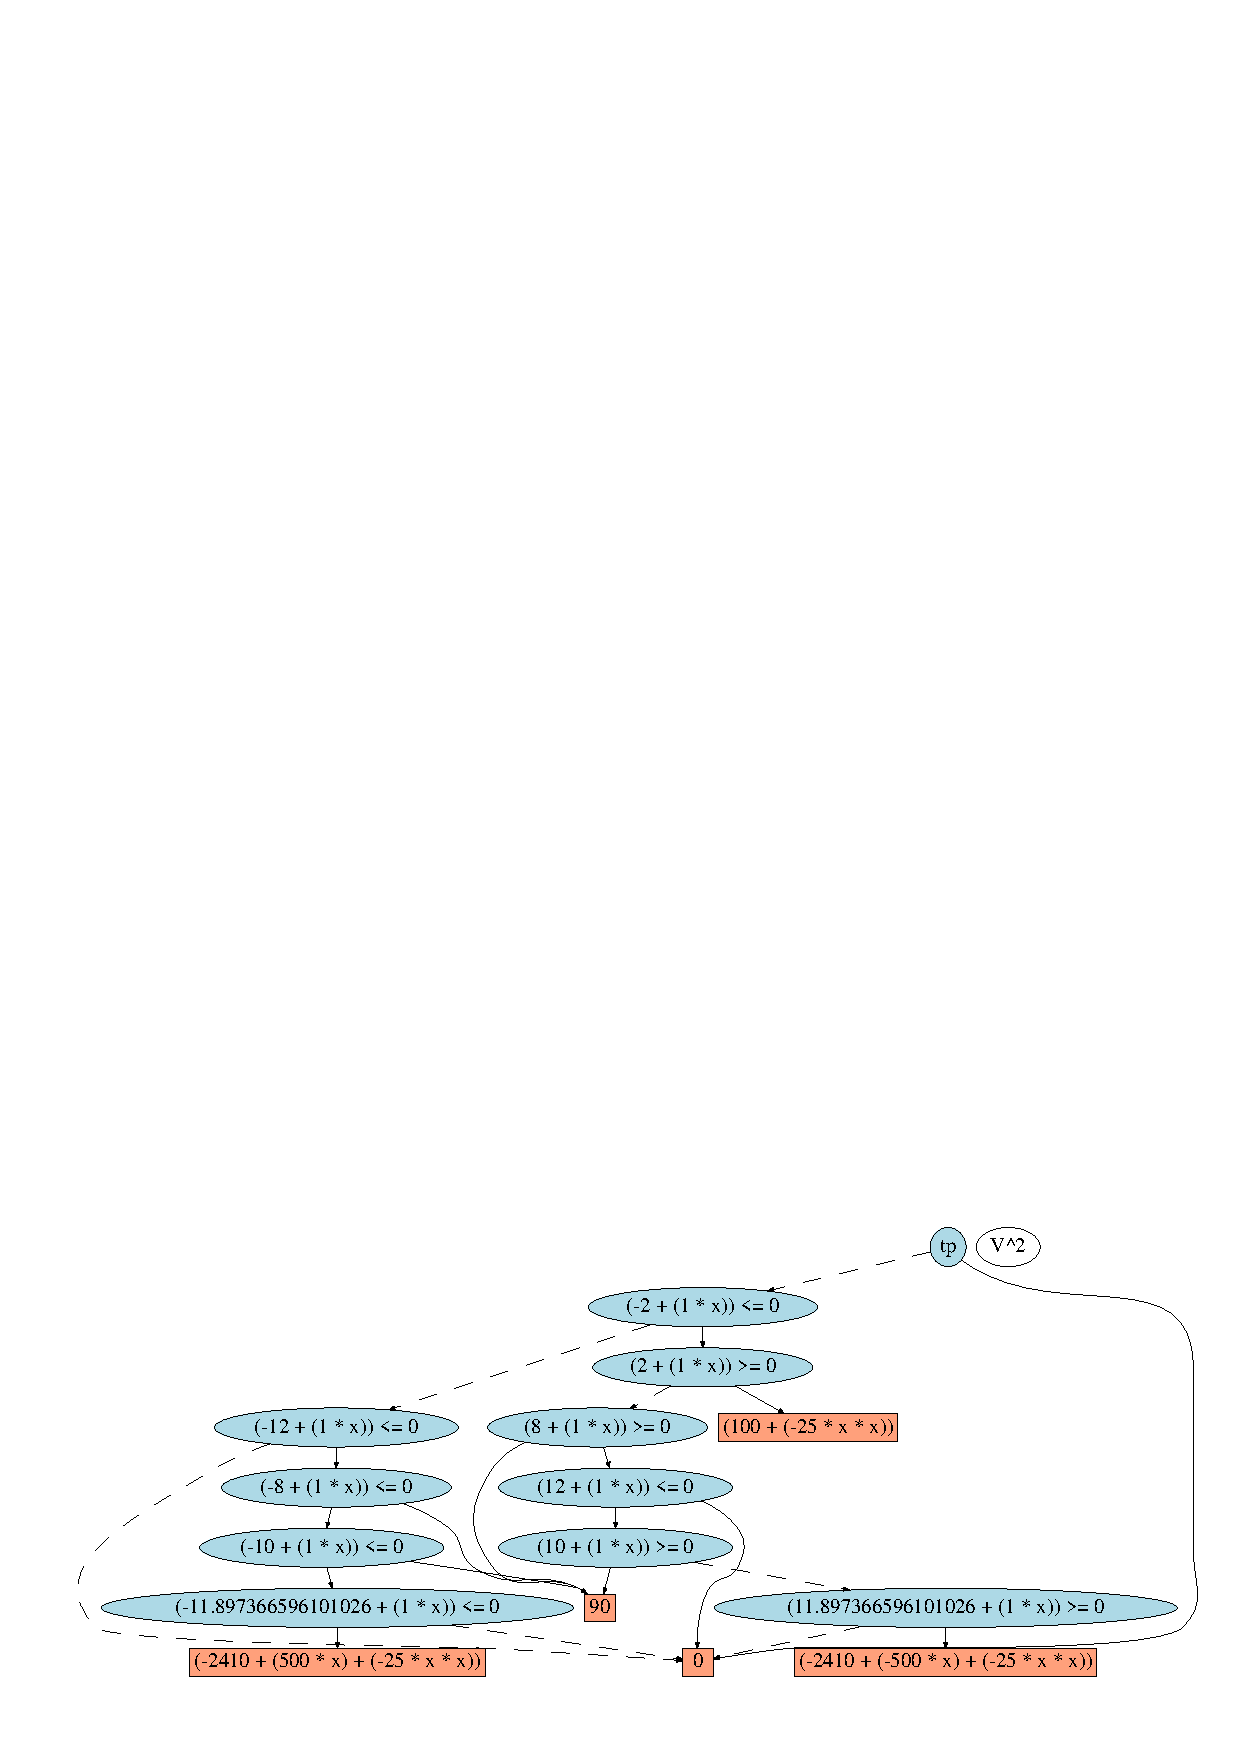
\includegraphics[width=0.4\textwidth]{Figures1/v2.pdf}
\end{center}
\vspace{-3mm}
\caption{%\footnotesize 
The final value function for the second horizon of the \MarsRoverNL example\
} \label{fig:rover_V2}
\vspace{-3mm}
\end{figure*}
%%%%%%%%%%%%%%%%%%%%%%%%%%%%%%%%%%%%%%%%%%%%%%%%%%%%%%%%%%%%%%%%%%%%%%%%%%

\section{Extended ADDs (XADDs)}

In practice, it can be prohibitively expensive to maintain
a case statement representation of a value function with explicit
partitions.  Motivated by the SPUDD~\cite{spudd} algorithm which
maintains compact value function representations for finite discrete
factored MDPs using algebraic decision diagrams (ADDs)~\cite{bahar93add},
we extend this formalism to handle continuous variables in a data
structure we refer to as the XADD.  An example XADD for the optimal
\MarsRoverNL value function for horizon 2 is provided
in Figure~\ref{fig:rover_V2}.


In brief we note that an XADD is like an ADD except that (a) the decision
nodes can have arbitrary inequalities, equalities, or disequalities (one
per node) and (b) the leaf nodes can represent arbitrary functions.
The decision nodes still have a fixed order from root to leaf
and the standard ADD
operations to build a canonical ADD (\textsc{Reduce}) and 
to perform a binary operation on two ADDs (\textsc{Apply}) 
still applies in the case of XADDs.

While exact solutions using symbolic dynamic
programming are possible in principle for arbitrary symbolic CSE transition
and reward functions, we note that it is much more difficult to
devise a canonical and compact form for representations 
such as~\eqref{eq:expr_reward}
in comparison to~\eqref{eq:simple_reward}.
Hence while we have used general examples throughout the paper
to demonstrate the expressiveness of our approach, we will restrict
XADDs to use \emph{polynomial} functions only.  We note the main advantage
of this for the XADD is that we can put the leaf and decision nodes
in a \emph{unique, canonical} form, which allows us to minimize 
redundancy in the XADD representation of a case statement.

It is fairly straightforward for XADDs to support all case operations
required for SDP.  Standard operations like unary multiplication,
negation, $\oplus$, and $\otimes$ are implemented exactly as they
are for ADDs.  The fact that the decision nodes have internal structure
is irrelevant, although this means that certain paths in the XADD
may be inconsistent or infeasible (due to parent decisions).  To
remedy this, when the XADD has only linear decision 
nodes, we can use the feasibility checkers of
a linear programming solver (e.g., as also done in~\cite{penberthy94}) 
to prune unreachable nodes in the XADD; later we show results demonstrating
impressive reductions in XADD size using this style of pruning.

The only two XADD operations that pose difficulty are substitution
and maximization.  In principle substitution is simple, the only
caveat is that substitutions modify the decision nodes and hence
decision nodes may become unordered.  We can use the 
recursive application of ADD binary operations $\otimes$ and $\oplus$ 
as given in Algorithm~\ref{fig:correct} to correctly reorder the
nodes in an XADD $F$ after substitution.  A related reordering
issue occurs during XADD maximization; because XADD maximization
can introduce new decision nodes (which occurs at the leaf when
two leaf functions are compared) and these decision nodes may
be out of order w.r.t.\ the diagram, reordering as defined
in Algorithm~\ref{fig:correct} must also be applied after
maximization.  

On a final note, we mention that an implementation of SDP using case
statements without any attempt to merge and simplify cases often
cannot get past the first or second SDP iteration; as our results show
next, XADDs allow SDP to scale to much longer horizons in practice.

%%%%%%%%%%%%%%%%%%%%%%%%%%%%%%%%%%%%%%%%%%%%%%%%%%%%%%%%%%%%%%%%%
\incmargin{1em}
%\linesnumbered
\begin{algorithm}[t!]
\SetKwFunction{getCanonicalNode}{{\sc GetCanonicalNode}}
\SetKwFunction{reduce}{{\sc Reorder}}
\SetKwInOut{Input}{input}
\SetKwInOut{Output}{output}

\Input{$F$ (root node for possibly unordered XADD)}
\Output{$F_r$ (root node for an ordered XADD)}
\BlankLine
\Begin{
   //if terminal node, return canonical terminal node\\
   \If{F is terminal node}
   {
   \Return{canonical terminal node for polynomial of $F$}\;
   }
   //nodes have a $\mathit{true}$ \& $\mathit{false}$ branch and $\mathit{var}$ id\\
   \If{$F \rightarrow F_r$ is not in Cache}
   {
    $F_{\mathit{true}}$ = \reduce{$F_{\mathit{true}}$} $\otimes \; \mathbb{I}[F_\mathit{var}]$ \;
    $F_{\mathit{false}}$ = \reduce{$F_{\mathit{false}}$} $\otimes \; \mathbb{I}[\neg F_\mathit{var}]$\;
    $F_r = F_{\mathit{true}} \oplus F_{\mathit{false}}$\;
    insert $F \rightarrow F_r$ in Cache\;
   } 
   \Return{$F_r$}\;
}
\caption{{\sc Reorder}(F)  \label{fig:correct}}
\end{algorithm}
\decmargin{1em}
%%%%%%%%%%%%%%%%%%%%%%%%%%%%%%%%%%%%%%%%%%%%%%%%%%%%%%%%%%%%%%%%%

\section{Empirical Results}


We implemented the SDP algorithm using the XADDs and tested it on several domains. Apart from the \MarsRoverNL,  we considered problems from the OR literature such as \InventoryControl  and \WaterReservoir. In the following subsections we will study these examples empirically.

%%%%%%%%%%%%%%%%%%%%%%%%%%%%%%%%%%%%%%%%%%%%%%%%%%%%%%%%%%%%%%%%%%%%%%%%%%
%figure5 : time-iteration and space-iteraton for 1d-2d-noPrune inventory
\begin{figure*}[t]
\centering
%\subfigure{
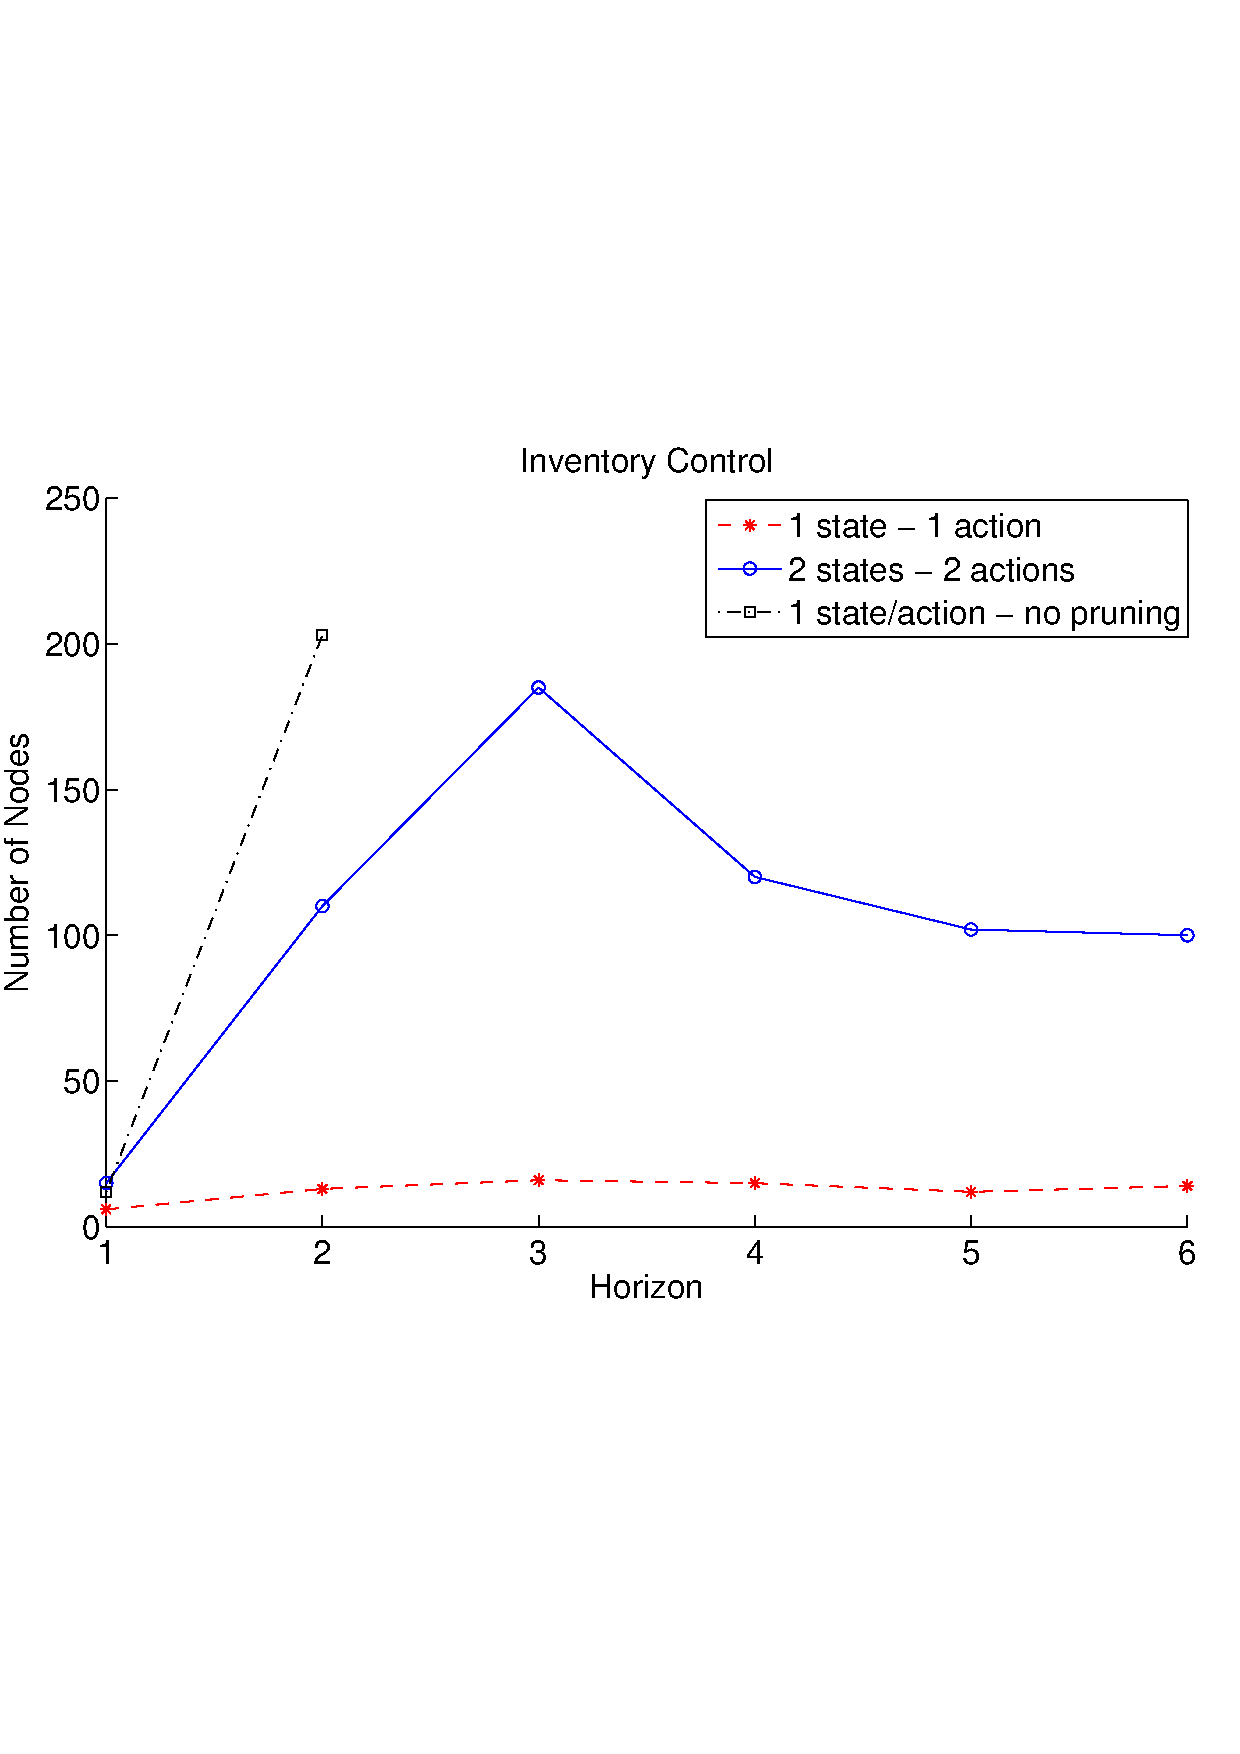
\includegraphics[width=0.47\textwidth]{Figures1/space1-3.pdf}
\hspace{5mm}
\includegraphics[width=0.47\textwidth]{Figures1/time1-3.pdf}
%}
%\vspace{-3mm}
\caption{%\footnotesize 
Space (\# XADD nodes in value function) and
time for different horizons of CSA-DP on \InventoryControl\ 
Comparing 1D, 2D and no-pruning}
\label{fig:invC}
%\vspace{-3mm}
\end{figure*}
%%%%%%%%%%%%%%%%%%%%%%%%%%%%%%%%%%%%%%%%%%%%%%%%%%%%%%%%%%%%%%%%%%%%%%%%%%

\subsection{\InventoryControl} 
This domain problem is a well-known optimization benchmark in the OR literature. Business firms often deal with the problem of deciding  upon the amount of product to order in a time period so that the customer demands are satisfied. The firm's warehouse will keep an inventory of this product to address different customer demand levels. Each month, the firm must decide on the amount of products to order based on the current stock level.
The order should not be too high since keeping the inventory is expensive, nor should it be too low in which case it will be penalized for being unable to meet customer demands and leading to the loss of customers. The optimization problem faced by the firm is to find an optimal order policy that maximizes the profit.~\cite{Mahootchi2009}

We present a simple formulation of this problem where the capacity of the inventory is C units of each product and customer orders not satisfied in this month are backlogged for the next month, so inventory can take negative values. We consider two cases, a one product inventory with one order action and the other with two products that needs two different orders.

We take two continuous state variable $x_1,x_2 \in [-1000,C]$ indicating the current inventory quantity into account, with the total inventory capacity of 800, and a stochastic boolean state variable for customer demand level $d$ where $d=0$ is low demand levels (50) and $d=1$ is high demand levels (150) according to some probability. \\
The continuous action variable is the order quantity $a_1,a_2 \in [0,C]$ which can at most take the value of the maximum inventory capacity. \\

We define an immediate negative reward for the cost of producing an order and the storage cost of holding the products in the inventory and also a positive reward for fulfilling the customer demand whenever there are enough stocks in the inventory. The transition for one of the state variables and the reward function are defined below:
%\ because of backlogging, the customer demand is always taken from the current stock level, leaving it negative
%\ consider the next state as the current state and orders minus the customer orders
%\ customer demands are boolean of low and high that change in every iteration
%\ 

{\footnotesize
\begin{align*}
x'_1 & = \begin{cases}
d  \wedge (x_1 + a_1 + x_2 - 150 \leq 800) : & x_1 + a_1 - 150 \\
d  \wedge (x_1 + a_1 + x_2 - 150 \geq 800) : & x_1 - 150  \\
\neg d \wedge (x_1 + a_1 + x_2 - 150 \leq 800): & x_1 + a_1 - 50    \\
\neg d \wedge (x_1 + a_1 + x_2 - 150 \geq 800): & x_1 - 50    \\
\end{cases}\\
d' & =  \begin{cases}
d     : &(0.7)\\
\neg d: &(0.3)\\
\end{cases}\\
R & = \begin{cases}
(x_1 + x_2 \geq 900) \wedge d\\
150 - 0.5\cdot a_1 -0.4 \cdot a_2 - 0.1\cdot(x_1 + x_2) \\
(x_1 + x_2 \leq 900) \wedge d\\
(150 - (x_1+x_2)) - 0.5\cdot a_1 -0.4 \cdot a_2 - 0.1\cdot(x_1 + x_2) \\
(x_1 + x_2 \geq 300) \wedge \neg d\\
50 - 0.5\cdot a_1 -0.4 \cdot a_2 - 0.1\cdot(x_1 + x_2) \\
(x_1 + x_2 \leq 300) \wedge \neg d\\
(50 - (x_1+x_2)) - 0.5\cdot a_1 -0.4 \cdot a_2 - 0.1\cdot(x_1 + x_2) \\
\end{cases}
\end{align*}}

% write description in case we have to take this huge case out! 
The transition for the continuous actions partitions based on the maximum capacity of the inventory (for both products), and only adds the orders if the current total capacity (with respect to the orders of that product and the stocks available for both products) are less than this maximum capacity. 

The demand variable is transitioned stochastically and the reward function is based on the demand levels and the current stock in inventory. If the current stock is larger than the total inventory, we get the reward for fulfilling the demand $(e.g 150)$, if the demand is high and the inventory is not high enough, then the reward is $(e.g (150 - (x_1+x_2)))$, in both cases the action costs and holding costs are also added. This allows the inventory to stock as many products as possible while not exceeding the capacity of the inventory. 

We plot the results of comparing a 1-product \InventoryControl problem with a multi-dimensional one. Figure~\ref{fig:invC} compares the time and nodes for different iterations for these two problem instances and a third comparisoon for the effect of not pruning on the 1D instance. This demonstrates the impact of having multiple constraints and action variables on the problem size which requires much more state-action partitions. The time and space have increased from the first iteration up to the third iteration for the 2D problem size, but then dropped for the next horizons due to pruning the XADD in our algorithm. As more constraints got added in for horizon 4, they cancelled the effects of some of the previous branches because of infeasibility and the pruning operation allows the XADD to grow smaller in space and requiring almost a constant time depending on the constraints added in each horizon. Without considering pruning, even the 1 product problem instance quickly falls into the curse of dimensionality problem. In fact, after the second iteration time and space grows exponentially and for this reason the plot fails to show the next time and space. 
% any need for 3d plot? For the 1 or 2 product case?
% any thing else we need from this example?



\subsection{\WaterReservoir}The problem of \WaterReservoir needs to make an optimal decision on how much and when to discharge water from water reservoirs to maximize hydroelectric energy productions while considering environment constraints such as irrigation requirements and flood prevention. 
A multi-reservoir system is more desirable than the single reservoir problem due to its ability in controlling various environment parameters such as flooding.  In these systems, the inflow of downstream reservoirs are effected by the outflow of their upstream reservoirs. In the OR literature, this case  is considered much more complex and for the sake of simplicity mainly the single case in considered. For multi-reservoirs the main problem that leads to approximations to DP methods or using other simplifications is the curse of dimensionality. In this domain the discharge action is considered as a discrete action  and so are the energy demands. This causes the state space to grow exponentially in case of multiple states and actions. ~\cite{reservoir}
Using our method for continuous action value iteration, we show that this problem can be handled efficiently and is scalable to multi-reservoir problems. Consider a two-level reservoir with the outflow of the second reservoir added to the input of the first reservoir. The state space is the level of water in both reservoirs as well as the energy demands and inflow (such as rainfall or streams) to the reservoirs $(l1,l2,i,e)$. We consider the water levels as continuous variables, the inflows to both reservoirs are the same which depends on a high-low sessions of rainfall. The energy demands e can be considered both continuous or discrete for different customer needs. 

We want to prevent the upstream reservoir ($l2$) from reaching low water levels, while avoiding flooding which is caused by high water levels. A constant amount of water is discharged from the downstream reservoir($l1$) to meet customer electricity demands. The inflow to both reservoirs is assumed to be the same (same amount of rainfall). 
{\footnotesize
\begin{align*}
l1' & = \begin{cases}
d     : & l1 - 1000 \cdot e + 500 \cdot e  +450 \cdot e \\
\neg d: &  l1 - 1000 \cdot e + 500 \cdot e  +250 \cdot e \\
\end{cases}\\
l2' & =  \begin{cases}
d     : & l2 - 500 \cdot e  +450 \cdot e \\
\neg d: &  l2 - 500 \cdot e  +250 \cdot e \\
 \end{cases}\\
d' & = \begin{cases}
d     : & (0.7) \\
\neg i: &  (0.3)   \\
\end{cases}\\
\end{align*}}

The reward is assigned based on preventing the flood. If water levels prevent flooding, a reward is given for the \textit{time} the reservoir selects the action of discharging water from one reservoir to the other($l2 to l1$), or the choice of not discharging at that time, depending on the water levels. The elapsed time is used as the reward value if the constraints are met, in this case the system should choose to perform an action (drain or no drain) as latest as possible. 
This elapsed time is added to the current time at each transition. The water levels are transitioned based on the previous levels and the amount of discharge and inflow multiplied by the elapsed time. This means that higher elapsed time is desired to maximize the reward, while lower ones ensure flood prevention.

{\footnotesize
\begin{align*}
R & = \begin{cases}
l1 \leq 4500 \wedge l2 \leq 4500 \wedge   l1\geq 50 : e \\
l1 \leq 4500 \wedge l2 \leq 4500 \wedge   l1\leq 50 : -100+e \\
\neg(l1 \leq 4500 \wedge l2 \leq 4500) : 0 \\
\end{cases}
\end{align*}}

In order to demonstrate the effectiveness of planning optimally with our model, we use this continuous-time example of the multi-reservoir where the elapsed time is defined as the action parameter to drain a reservoir. The goal is to show a form of value function refinement that is generated using this CSA-DP algorithm. The optimal value function will obtain higher values for higher horizons, while the value for lower horizons were less than the current value function. This is demonstrated in Figure~\ref{fig:reservoir} where three value functions have been presented in different horizons. 

Here flood prevention is ensured in each step by the linear piecewise boundaries on the very high and very low levels, the action of discharging occurs here either at time 0 for very critical points or at a time depending on the water levels later during the iteration (i.e, $a = -8.18 + 0.0018*l1$ if one of the water levels is above the critical level in the third iteration). As for the constant section, this piece is the safe range and the action of discharge (or not discharge) is left till the latest possible time thus achieving higher rewards. As the iteration number increases, the future discounted reward goes higher than the previous horizon. 

%%%%%%%%%%%%%%%%%%%%%%%%%%%%%%%%%%%%%%%%%%%%%%%%%%%%%%%%%%%%%%%%%%%%%%%%%%
%figure6 : 3d plots of refinement planning for 3 horizons
\begin{figure*}[t]
\centering
\includegraphics[width=0.33\textwidth]{Figures1/ref1.pdf}
\includegraphics[width=0.33\textwidth]{Figures1/ref3.pdf}
\includegraphics[width=0.33\textwidth]{Figures1/ref6.pdf}
\caption{%\footnotesize 
Exact optimal value function for \WaterReservoir  domain
}
\label{fig:reservoir}
%\vspace{-3mm}
\end{figure*}
%%%%%%%%%%%%%%%%%%%%%%%%%%%%%%%%%%%%%%%%%%%%%%%%%%%%%%%%%%%%%%%%%%%%%%%%%%

\section{Related Work}
The most relevant vein of Related work is that of~\cite{feng04}
and~\cite{li05} which can perform exact dynamic programming on
DC-MDPs with rectangular piecewise linear reward and transition functions
that are delta functions.  While SDP can solve these same problems,
it removes both the rectangularity and piecewise restrictions on the
reward and value functions, while
retaining exactness.  
Heuristic search approaches with formal guarantees 
like HAO*~\cite{hao09} are an attractive future extension of SDP;
in fact HAO* currently uses the method of~\cite{feng04}, which could
be directly replaced with SDP.  While~\cite{penberthy94} has considered
general piecewise functions with linear boundaries (and in fact,
we borrow our linear pruning approach from this paper), this work
only applied to fully deterministic settings, not DC-MDPs.

Other work has analyzed limited DC-MDPS having only one continuous
variable.  Clearly rectangular restrictions are meaningless with
only one continuous variable, so it is not surprising that more
progress has been made in this restricted setting.  One continuous
variable can be useful for optimal solutions to time-dependent MDPs 
(TMDPs)~\cite{boyan01}.  Or phase transitions can be used to 
arbitrarily approximate one-dimensional continuous distributions
leading to a bounded approximation approach for arbitrary single continuous
variable DC-MDPs~\cite{phase07}.  
While this work cannot handle arbitrary stochastic
noise in its continuous distribution, it does exactly solve DC-MDPs
with multiple continuous dimensions.

Finally, there are a number of general DC-MDP approximation
approaches that use approximate linear programming~\cite{kveton06}
or sampling in a reinforcement learning style approach~\cite{munos02}.
In general, while approximation methods are quite promising in
practice for DC-MDPS, the objective of this paper was to push
the boundaries of \emph{exact} solutions; however, in some sense, 
we believe that more expressive exact solutions may also inform
better approximations, e.g., by allowing the use of data structures
with non-rectangular piecewise partitions that allow higher fidelity
approximations.

\section{Conclusions}


\bibliography{exact_sdp}
\bibliographystyle{aaai}
\end{document}
